%%%%%%%%%%%%%%%%%%%%%%%%%%%%%%%%%%%%%%%%%%%%%%%%%%%%%%%%%%%%%%%%%%%%%%%
%                          template.tex
%
% LaTeX template for papers conforming to the United States Sections of
% the Combustion Institute style guide.
%
% Authors:
%     Bryan W. Weber, University of Connecticut
%     Kyle E. Niemeyer, Oregon State University
%
% This work is licensed under the Creative Commons Attribution 4.0
% International License. To view a copy of this license, visit
% http://creativecommons.org/licenses/by/4.0/.
%%%%%%%%%%%%%%%%%%%%%%%%%%%%%%%%%%%%%%%%%%%%%%%%%%%%%%%%%%%%%%%%%%%%%%%

\documentclass[12pt]{ussci}

%======================================================================
% packages
\usepackage{textgreek}
\usepackage{amsmath,amsfonts,amssymb}
\usepackage{graphicx}
\usepackage{float}
\restylefloat{table}
\usepackage{booktabs} % for much better looking tables
\usepackage{array} % for better arrays (eg matrices) in maths
\usepackage{paralist} % very flexible & customisable lists (eg. enumerate/itemize, etc.)
\usepackage{listings}
\usepackage{verbatim} % adds environment for commenting out blocks of text & for better verbatim
\usepackage{caption}
\usepackage{subcaption} % make it possible to include more than one captioned figure/table in a single float
\usepackage{multirow}
\usepackage{rotating}
\usepackage{ulem}
\usepackage{bigstrut}
\usepackage{bm}
\usepackage[space]{grffile}
\usepackage{tikz}
\usetikzlibrary{shapes.geometric, arrows}
\usetikzlibrary{calc,patterns,angles,quotes,shapes,positioning}
\usepackage{xspace}
\usepackage{enumitem}
\usepackage[version=4]{mhchem}

%better printing of numbers
\usepackage[T1]{fontenc}
\usepackage[english]{babel}
\usepackage{csquotes}
\usepackage{textcomp}

\usepackage{siunitx}
\sisetup{group-separator={,},
     detect-all,
     binary-units,
     list-units = single,
     range-units = single,
     tophrase = --,
     per-mode = symbol-or-fraction,
     separate-uncertainty = true,
     list-final-separator = {, and }
%    scientific-notation = fixed
}
\DeclareSIUnit\atm{atm}

\newcommand{\degree}{\ensuremath{{}^{\circ}}\xspace}
\usepackage{listings}
\usepackage{blindtext}
\usepackage{subfiles}
\usepackage{breakcites}
%======================================================================
% Add your bibliography file here, replace template.bib
\addbibresource{mendeley.bib}
%======================================================================
% Replace "Reaction Kinetics" in the line below by your paper topic
\newcommand\papertopic{Reaction Kinetics}
%======================================================================

\graphicspath{{./Figures/}}

\title{ Investigating stiffness detection metrics for chemical kinetics }

\author[1]{Andrew Alferman}
\author[1,*]{Kyle E. Niemeyer}


\affil[1]{School of Mechanical, Industrial, and Manufacturing Engineering\\
		Oregon State University, Corvallis, OR 97331, USA}
\affil[*]{Corresponding author: \email{Kyle.Niemeyer@oregonstate.edu}}


\begin{document}
\maketitle

%====================================================================
\begin{abstract} % not to exceed 200 words

%Abstract should be between 150--200 words and should state briefly the purpose of the research, the principal results and major conclusions. An abstract is often presented separately from the article, so it must be able to stand alone. For this reason, References should be avoided, but if essential, then cite the author(s) and year(s). Also, non-standard or uncommon abbreviations should be avoided, but if essential they must be defined at their first mention in the abstract itself.

Simulations of combustion and reacting flows often encounter stiffness in the equations governing chemical kinetics.
Explicit solvers for these ordinary differential equations offer low computational expense, but typically cannot efficiently handle stiff systems.
In contrast, implicit methods demand greater expense but offer unconditional stability\textendash as a result, most reactive flow solvers rely on these methods by default (other than explicit direct numerical simulation solvers).
However, explicit or stabilized explicit methods can instead be used to reduce the computational expense while remaining stable and accurate if the chemical kinetics systems exhibit low-to-moderate stiffness.
This study investigates metrics for quantifying stiffness, with the goal of identifying one capable of efficiently and robustly determining the appropriate category of integrator required.
Methods of measuring the stiffness of chemical kinetics states will be investigated, including stiffness ratio, stiffness index, stiffness indicator, and chemical explosive mode.
These will be applied to simulations of hydrogen/carbon monoxide and methane autoignition using initial conditions representative of realistic turbulent combustion, obtained from partially stirred reactor simulations.
The stiffness quantification metrics will be compared with the time required to integrate using implicit and explicit methods.
We will conclude by analyzing preliminary performance analysis of an integrator scheduler using these metrics.

\end{abstract}

% Provide 2-4 keywords describing your research. Only abbreviations firmly
% established in the field may be used. These keywords will be used for
% sessioning/indexing purposes. Use \sep between each keyword.
\begin{keyword}
    Stiffness quantification\sep Ordinary differential equations\sep Chemical kinetics\sep Computational cost reduction
\end{keyword}

%====================================================================
\section{Introduction}
%

An increasing demand for greater efficiency and lower \ce{CO2} emissions in the US energy supply has driven the development of next-generation combustion technologies that use alternative fuels \cite{Epstein2012}.
Computational modeling is one important tool that increasingly drives design and development of these new technologies.
Shortening the design cycle and time-to-market of novel and efficient energy devices optimized for alternative fuels requires fundamental advances in combustion science and fuel chemistry; both depend on high-fidelity computational tools~\cite{Niemeyer}.
The need to develop new, high-performance computational methods to support combustion research has been recognized by multiple federal agencies as a key objective towards implementing predictive models~\cite{Trouve:2006tq,DOE:2007tj,NationalResearchCouncil:2011ub,National-Research-Council:2014aa}.

Species time scales can range from the order of nanoseconds to seconds, requiring greater computational expense for integration by conventional methods (i.e., numerical stiffness)~\cite{Lu2009}.
Most combustion modeling approaches rely on a single, implicit ODE integration method to handle the chemistry in all spatial locations, but these methods are computationally expensive, especially for larger mechanisms.
The computational cost of chemistry is either a quadratic or cubic function of the number of species~\cite{Lu2009}; reaction mechanisms of sizes comparable to those shown above pose computational difficulties even in zero-dimensional (homogeneous) simulations.

Depending on the local conditions, computational flow time-step size, and chemical mechanism being used, it is possible to encounter a wide range of stiffness within a single simulation.
We can exploit this situation to reduce the overall simulation expense by selecting the most computationally efficient ODE solver on-the-fly based on local conditions.
For example, a low-cost explicit method may be used far away from the reaction zone, while an implicit---or otherwise ``stiff''---solver is more economical inside a flame.
Making this selection requires a method to detect and classify stiffness~\cite{Niemeyer}.

Although the concept of stiffness has been identified for over 60 years, the term has not been precisely defined despite repeated efforts.
The diverse set of problems considered to be ``stiff'' and the large variety of characterizations used to describe stiffness are amongst the difficulties that have been encountered in developing a precise definition~\cite{Soderlind2014}.
Nonetheless, a variety of stiffness quantification methods have been developed with the goal of providing a practical means of evaluating a systems ODEs~\cite{Soderlind2014,Shampine1985,Brugnano2011,Lambert1973ComputationalEquations,Hairer1996SolvingII}.
We look to these methods of stiffness quantification to determine their usefulness with respect to the equations governing combustion, and to determine if a reliable and efficient means of switching methods can be developed from it.
In doing so, we hope to reduce the computational expense of combustion simulations.

\section{Methods}
% REVIEW IF GRI MECH CAN'T BE COMPLETED IN TIME
We considered two different chemical kinetic models in this study: the relatively small hydrogen\slash carbon monoxide (\ce{H2}\slash \ce{CO}) model of Burke et al.~\cite{Burke:2011fh} and GRI Mech 3.0~\cite{grimech3}, which uses \ce{CH4} as fuel.
The \ce{H2}\slash \ce{CO} model uses 13 species while the GRI Mech 3.0 is larger and uses 53 species, allowing for Jacobian matrices of system of ODEs of $13 \times 13$ and $53 \times 53$, respectively.
These relatively small Jacobian matrices allow for much faster evaluations of stiffness than would be possible with larger, more complicated kinetic systems, which can have hundreds to hundreds of thousands of chemical species~\cite{Niemeyer:2013}.

The code used to run autoignition simulations and calculate stiffness metrics was written in Python and made use of open-source software, including the \texttt{ode} integrator function of SciPy~\cite{SciPy}.
Two different integrators of the \texttt{ode} integrator function were used: the implicit \texttt{vode} integrator, which uses an implicit Adams method for non-stiff problems and a method based on the backwards differentiation formulae (BDF) for stiff problems~\cite{Brown1989}, and the explicit \texttt{dopri5} integrator, which uses a Runge-Kutta method of order (4)5 developed by Dormand and Prince with automatic step size control~\cite{E.HairerSPNorsett1990}.
The \texttt{vode} integrator was set to use the default behavior of using first-order finite differencing to provide an estimate of the Jacobian matrix.
\texttt{NumPy}~\cite{VanDerWalt2011} was also extensively used in the code to determine eigenvalues and perform numerous basic mathematical functions.
To ensure a high degree of accuracy, the integrator was given values of \num{e-15} and \num{e-17} for the error control parameters \texttt{relerr} and \texttt{abserr}, respectively.

Computation of the right hand side (RHS) function and the Jacobian matrix of the systems of ODEs were readily achieved using pyJac~\cite{pyJac:1.0.2}, a Python-based open-source program that generates analytical Jacobian matrices for use in chemical kinetics modeling and analysis~\cite{Niemeyer:2017}.
pyJac uses a chemical mechanism developed using Cantera~\cite{Goodwin:2015aa} software and a set of initial conditions to generate functions that return the required values.  A global variable was added to the RHS function to count the number of calls from the integrator for each time-step.

Our analysis was conducted using information gathered from partially stirred reactor (PaSR) simulations.
As described by Niemeyer et al.~\cite{Niemeyer:2017}, the PaSR model consists of a number of particles, each with a time-varying composition.
At discrete time-steps, events including inflow, outflow, and pairing cause particles to change composition; between these time-steps, mixing and reaction fractional steps evolve the composition of all particles.
By using data from a single particle of the PaSR model, the evaluation could be simplified to a zero-dimensional analysis.
The \ce{H2}\slash \ce{CO} simulation used a different set of PaSR data than the GRI Mech 3.0 simulation.
Both sets of PaSR data included nine different configurations of temperature and pressure; the initial temperature values were 400, 600, and 800 K, while the pressure values were 1, 10, and 25 atm.
Pressure remained constant throughout the simulations.

% Not sure why this one is here.
% (Please refer to Niemeyer et al.~\cite{Niemeyer:2017} for a detailed description of the relevant equations and solution technique.)

% To ensure that the code was running properly, the van der Pol equation with a \(\epsilon\) value of 1000 was used as a test equation.

The four stiffness quantification methods discussed within this paper are the stiffness ratio, the stiffness index, the stiffness indicator, and the chemical explosive mode.
Variable names have been changed in the equations below to maintain consistency throughout this paper.

\subsection{Stiffness Ratio}
One commonly referenced measure of the stiffness of a system of ODEs is the ``stiffness ratio.''
The stiffness ratio of the system of ODEs is defined as
\begin{equation}
	\textrm{Stiffness Ratio} = \frac{\textrm{max}|\lambda_p|}{\textrm{min}|\lambda_p|}
\end{equation}
in which $\lambda_p$ is an eigenvalue of the Jacobian matrix of the system of ODEs~\cite{LeVeque2007}.
A large stiffness ratio is an indication of a large range of time scales in the problem, which is a necessary component for stiffness to arise.
This method is readily implemented and carries little computational cost beyond determining the eigenvalues of the Jacobian matrix.

\subsection{Stiffness Index}

One method of interest regarding stiffness quantification was the ``IA-Stiffness Index'' proposed by Shampine~\cite{Shampine1982}.
This method enables comparison of values of the stiffness index between different equations and different methods.
Additionally, the method takes into account the impact of the order of the method selected when evaluating the stiffness.
The method is relatively straightforward to implement, requiring computation of a vector of the derivatives of the system of equations, as well as either a weighted norm or the spectral radius of the Jacobian matrix.

% Replaced the Jacobian $f_y(x_n,y(x_n))$ with $A$ to keep consistent nomenclature
The IA-stiffness index of a method of order \textit{p} introduced by Shampine~\cite{Shampine1982} is
\begin{equation}
    \frac{h_{acc}}{h_{iter}} \doteq \tau ^ {1/(p + 1)} \rho [A] \|y^{(p+1)}(x_n)\|^{-1/(p+1)} \left( \frac{|\xi|^{-1/(p+1)}}{|\gamma|} \right)
\end{equation}
or alternatively,
\begin{equation}
    \frac{h_{acc}}{h_{iter}} \doteq \tau ^ {1/(p + 1)} \|A\|\|y^{(p+1)}(x_n)\|^{-1/(p+1)} \left( \frac{|\xi|^{-1/(p+1)}}{|\gamma|} \right)
\end{equation}
where $h_{acc}$ represents the largest step size which would result in a local accuracy test being passed, $h_{iter}$ represents the minimum step size that will lead to divergence of simple iteration, $\tau$ represents the specified tolerance, $\rho [A]$ represents the spectral radius of the Jacobian matrix $A$, $\gamma$ is a constant characteristic of the formula, and $\xi$ represents a constant characterizing the accuracy of a reference method.
Note that these equations require the $p+1$ derivative of the function $y(x_n)$.
Additionally, the matrix norm $\|M\|$ of matrix $M$ with $i$ columns and $j$ rows is given by
\begin{equation}
    \|M\| = \max_{i} \frac{1}{w_i} \sum_{j} |M_{ij}|w_j
\end{equation}
in which \(w_i\) and \(w_j\) are positive weights of the matrix~\cite{Shampine1985}.

Although the IA-stiffness index is useful in determining the stiffness of a method for a given system of equations, we are interested in quantifying the stiffness inherent to the system of equations itself.
Such a quantification is necessary for investigating method switching mechanisms.
Shampine notes that the scalar quantity
\begin{equation}\label{eqn:stiffness}
    \textrm{Stiffness Index} = \rho [A] \|y^{(p+1)}(x_n)\|^{-1/(p+1)}
\end{equation}
provides a fair ``stiffness index'' to a given problem~\cite{Shampine1985}. For the remainder of this document, all references to the stiffness index will refer to the value obtained using equation (\ref{eqn:stiffness}).
A large value of the stiffness index at a given point is an indication that the system of ODEs is locally stiff at that point.

As previously noted, use of the above equations requires calculation of a vector of the derivatives of a system of equations.
In the case of this investigation, this vector is comprised of the derivatives of the thermochemical composition vector with respect to time, with the the vector defined as
\begin{equation}
    \Phi = \{T, Y_1, Y_2, \dots, Y_{N_{sp}} \}^\intercal \;,
\end{equation}
where $T$ is the temperature, $Y_i$ are the species mass fractions, and $N_{sp}$ is the number of species in the mechanism~\cite{Niemeyer:2017}.
The vector needed to compute the stiffness index is therefore
\begin{equation}
    \frac{\partial \Phi}{\partial t} = \left\{\frac{\partial Y_1}{\partial t}, \frac{\partial Y_2}{\partial t}, \dots, \frac{\partial Y_{N_{sp}}}{\partial t} \right\}^\intercal \;,
\end{equation}
where time is denoted by $t$~\cite{Niemeyer:2017}.
In addition to this vector of derivatives, computation of the stiffness index requires either the weighted norm or the spectral radius of the Jacobian matrix for the thermochemical composition vector.

After generating this data using pyJac, the values of the second derivative of the thermochemical composition vector were calculated numerically using a fourth-order central differencing formula.
Numerical approximations of higher-level derivatives may also be generated using the same approach.
% REVIEW THIS
Use of the central differencing formula was possible because the stiffness index was calculated after solving for the thermochemical composition vector, and the reaction was modeled using time-steps of a constant size.
Forward and backward difference formulae were used at the boundaries where central differencing could not be used.
Variable time-step methods for calculating the second derivative or higher-level derivatives may also be used, however these methods were not necessary at the current stage of the investigation.

To facilitate comparison of the results obtained by Shampine~\cite{Shampine1985}, the order of the method was assumed to be 1 for all computations performed in this paper.

\subsection{Stiffness Indicator}
The ``stiffness indicator'' of a system of ODEs was proposed by S{\"o}derlind et. al. as a mathematically rigorous approach to characterize stiffness that works independent of the integration method used or operational criteria~\cite{Soderlind2014}.
S{\"o}derlind notes that ``large'' negative values of the stiffness indicator are a necessary condition for stiffness.
S{\"o}derlind further quantifies how ``large'' the negative values must be for an equation to be considered locally stiff for a given problem, however we are primarily interested in the values of the stiffness indicator itself to facilitate comparison between different simulations using different models and different timescales.

In the chemical kinetic models of interest, the stiffness indicator is calculated for a given Jacobian matrix $A \in \mathbb{R}^{n \times n}$ as:
\begin{equation}
	\textrm{Stiffness Indicator} = \frac{m[A] + M[A]}{2}
\end{equation}
where
\begin{equation}
	m[A] = \textrm{min}\,\lambda[\textrm{He}(A)];\qquad M[A] = \textrm{max}\,\lambda[\textrm{He}(A)],
\end{equation}
with $\lambda [A]$ denoting the eigenvalues of matrix $A$ and $\textrm{He}(A)$ denoting the Hermitian part of the matrix $A$, which is defined as
\begin{equation}
	\textrm{He}(A) = \frac{A + A^\intercal}{2}.
\end{equation}
While determination of the stiffness indicator does require calculation of eigenvalues following a transpose and addition of the Jacobian matrix, it is readily implemented and unlike the stiffness index it does not require storage of prior values of the solution.

\subsection{Chemical Explosive Mode}
The ``chemical explosive mode analysis'' (CEMA) was developed as a diagnostic to identify flame and ignition structure in complex flows~\cite{Yoo2009}.
Though this metric was not originally intended as a device to quantify the numerical stiffness of a system of ODEs, we are interested in determining if correlations exist between identification of the flame structure and the computational work required to advance the simulation for either explicit or implicit methods.
The chemical explosive modes are associated with positive eigenvalues of the Jacobian of the system of ODEs:
\begin{equation}
	\textrm{Re}(\lambda) > 0.
\end{equation}
Similar to the stiffness ratio, the CEMA is readily implemented and carries little computational cost beyond determining the eigenvalues of the Jacobian matrix.

\section{Results and Discussion}
% NEED TO UPDATE
%Initial conditions were picked using particles of the PaSR simulation where weak reactions were taking place but ignition had not yet occurred.
%The simulation was run until 0.2 seconds of data was obtained, in which time the particles exhibited autoignition.
%Using state data obtained during the simulation, the Jacobian matrix was calculated at each time-step using \texttt{pyJac}, which allowed the numerical values of each stiffness matrix to be calculated.

An analysis of each stiffness metric was performed using every particle in the PaSR simulation.
In this analysis, a simulation at each particle of the PaSR was advanced only as long as needed to obtain an accurate numerical value of each stiffness metric.
Because a fourth order central difference formula was used to numerically calculate the second derivatives in the calculation of the stiffness index, this resulted in five time-steps being used for each particle.
The only information needed to calculate the stiffness ratio, stiffness indicator, and chemical explosive modes is the Jacobian matrix, therefore these values could be calculated at every time-step as soon as the solution was known.
A constant step size of $1 \times 10^{-6}$ s was used for the computation, however the built in methods of the \texttt{ode} package have automatic step size control to ensure that values remain within tolerance, and the integrator may take many steps in between the specified time-step.
Using state data obtained during the simulation, the Jacobian matrix was calculated at each time-step using \texttt{pyJac}, which allowed the numerical values of each stiffness matrix to be calculated.
The code was configured to count the number of RHS function calls used by either \texttt{vode} or \texttt{dopri5} while integrating.

\subsection{Results}
%% NEED TO RUN DATA FOR CEMA OR OTHERWISE FIND THE PLOT
%\begin{figure}[htbp]
%    \centering
%    \begin{subfigure}{0.42\textwidth}
%        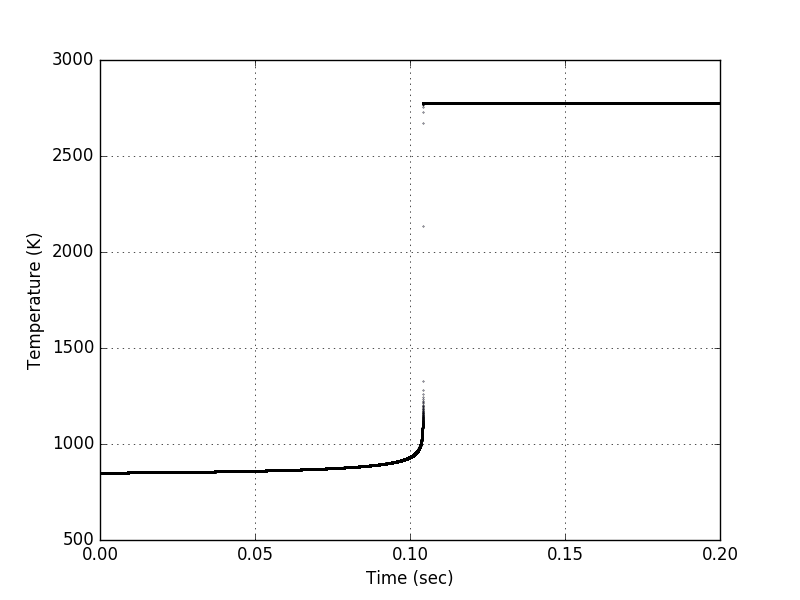
\includegraphics[width=\linewidth]{Autoignition_Temperature_1e-06_08_03.png}
%        \caption{The temperature of the simulation rises from approximately \SI{850}{\kelvin} prior to autoigniton to approximatley \SI{2775}{\kelvin}, with a residence time of approximately 0.10 seconds.}
%        \label{fig:tempcurveH2COAuto}
%    \end{subfigure}
%    \hfill
%    % NEED TO FIX LEGEND
%    \begin{subfigure}{0.42\textwidth}
%        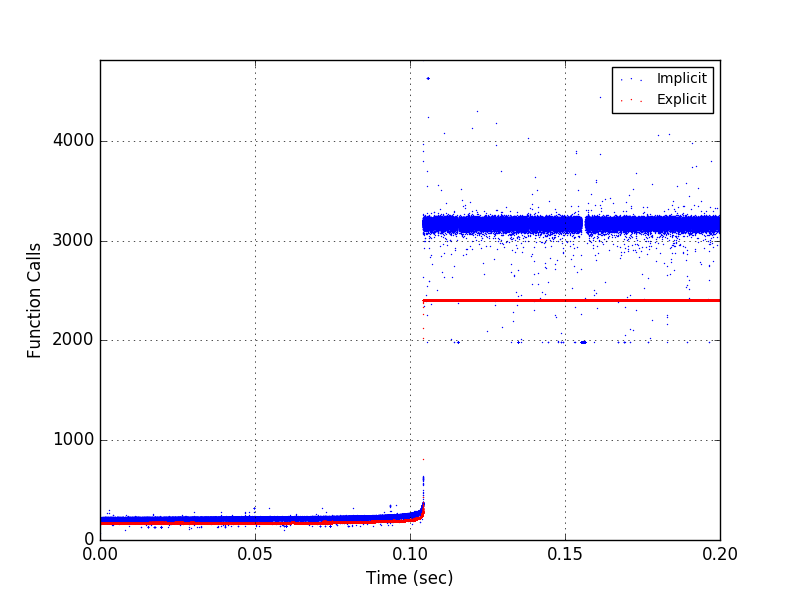
\includegraphics[width=\linewidth]{Autoignition_Function_Work_1e-06_08_17.png}
%        \caption{The number of RHS function calls per time-step increases slowly prior to autoignition and rapidly increases during ignition, then remains relatively constant and large after ignition.}
%        \label{fig:fnworkH2COAuto}
%    \end{subfigure}
%    \begin{subfigure}{0.42\textwidth}
%        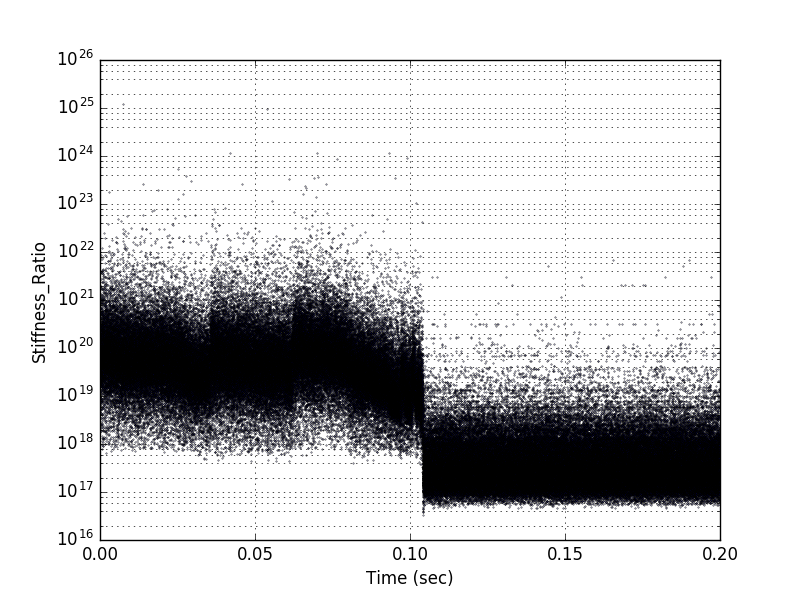
\includegraphics[width=\linewidth]{Autoignition_Stiffness_Ratio_1e-06_08_03.png}
%        \caption{The stiffness ratio remains large throughout the simulation, but decreases in magnitude after ignition.}
%        \label{fig:SRH2COAuto}
%    \end{subfigure}
%    \hfill
%    \begin{subfigure}{0.42\textwidth}
%        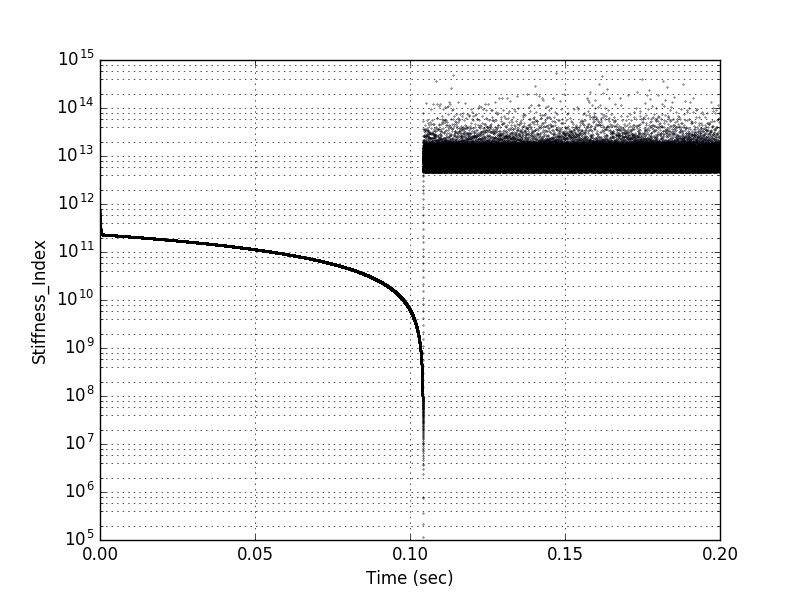
\includegraphics[width=\linewidth]{Autoignition_Stiffness_Index_1e-06_08_03.png}
%        \caption{The stiffness index slowly decreases prior to autoignition and increases following autoignition.}
%        \label{fig:SI1H2COAuto}
%    \end{subfigure}
%        \begin{subfigure}{0.42\textwidth}
%        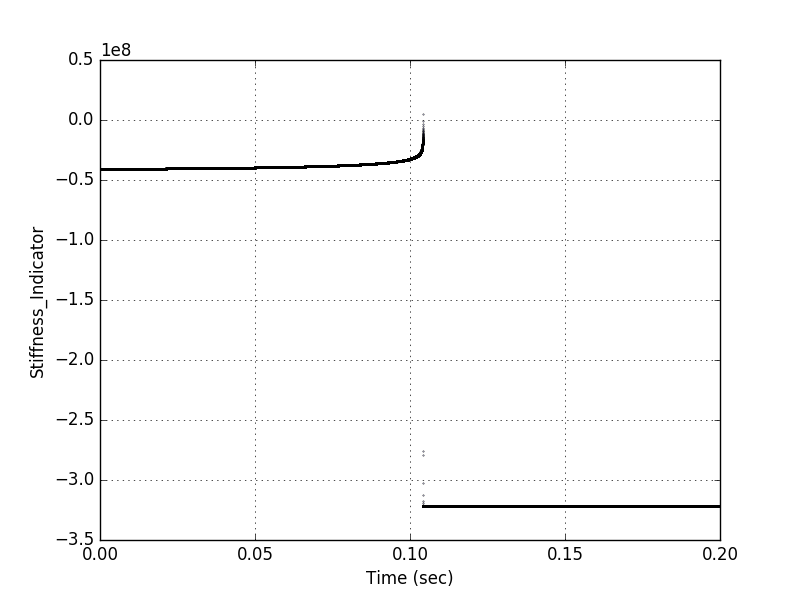
\includegraphics[width=\linewidth]{Autoignition_Stiffness_Indicator_1e-06_08_03.png}
%        \caption{A plot of the stiffness indicator resembles an upside down plot of RHS function calls.}
%        \label{fig:SI2H2COAuto}
%    \end{subfigure}
%    \caption{Temperature, RHS function calls, and stiffness metrics of the \ce{H2}\slash \ce{CO} reaction calculated with a constant step size of \SI{e-6}{\second}, integration time of \SIrange{0.0}{0.2}{\second}.}
%    \label{fig:H2COAutoStiffness}
%\end{figure}
The PaSR data for the \ce{H2}\slash \ce{CO} model consisted of 900900 different particles.
It was found that \texttt{vode} used fewer RHS function calls than \texttt{dopri5} for 139234 particles or 15.4\% of the PaSR data for this model, while \texttt{dopri5} used fewer function calls for 757569 particles or 84.0\% of the PaSR data.
\texttt{vode} and \texttt{dopri5} used the same number of function calls for 4097 particles, and \texttt{dopri5} did not fail at any particle in the \ce{H2}\slash \ce{CO} model.
A depiction of the number of function calls used by both \texttt{vode} and \texttt{dopri5} can be found in Figure~\ref{fig:FWH2COPaSR}.
In general, \texttt{vode} outperformed \texttt{dopri5} when pressure was 1 atm and at 400K while pressure was 10 atm.
At higher pressures and temperatures, the explicit \texttt{dopri5} generally outperformed the implicit \texttt{vode} when using this model.

\begin{figure}[htbp]
    \centering
    \begin{subfigure}{0.43\textwidth}
        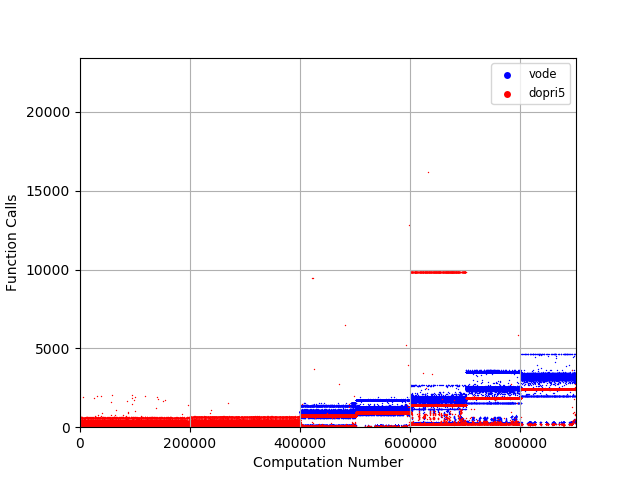
\includegraphics[width=\linewidth]{H2_CO/PaSR_Fn_Work_1e-06.png}
        \caption{Number of function calls used to integrate one time-step for both \texttt{dopri5} and \texttt{vode} at each particle of the PaSR model.}
        \label{fig:FWH2COPaSR}
    \end{subfigure}
    \hfill
    \begin{subfigure}{0.43\textwidth}
        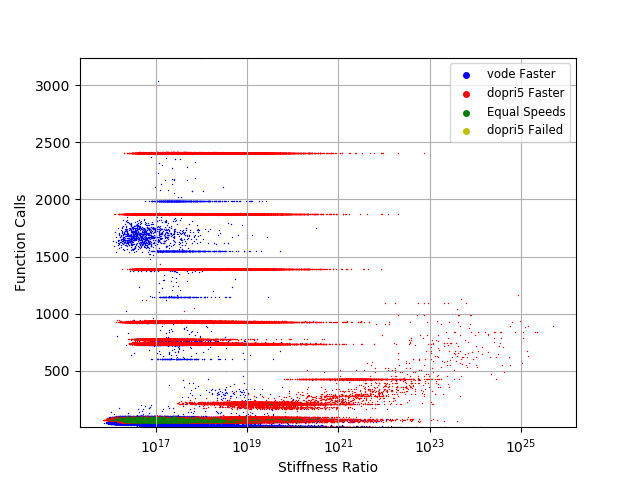
\includegraphics[width=\linewidth]{H2_CO/PaSR_Fn_Work_Ratio_Groupings_1e-06.png}
        \caption{Stiffness ratio versus the least function calls used to integrate one time-step at each particle of the PaSR model.}
        \label{fig:SRH2COPaSR}
    \end{subfigure}
    \begin{subfigure}{0.43\textwidth}
        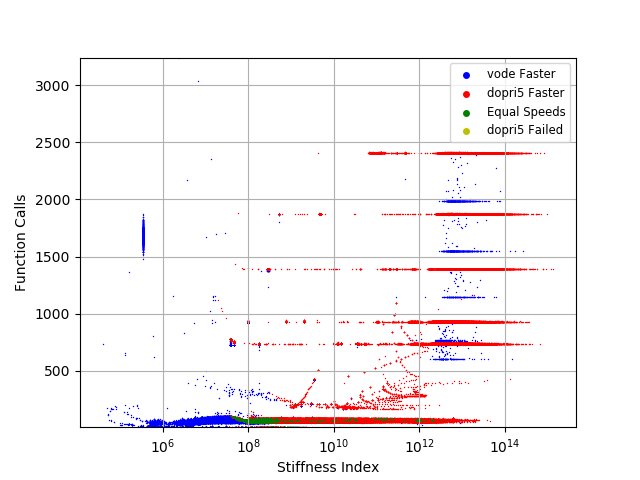
\includegraphics[width=\linewidth]{H2_CO/PaSR_Fn_Work_Index_Groupings_1e-06.png}
        \caption{Stiffness index versus the least function calls used to integrate one time-step at each particle of the PaSR model.}
        \label{fig:SI1H2COPaSR}
    \end{subfigure}
    \hfill
    \begin{subfigure}{0.43\textwidth}
        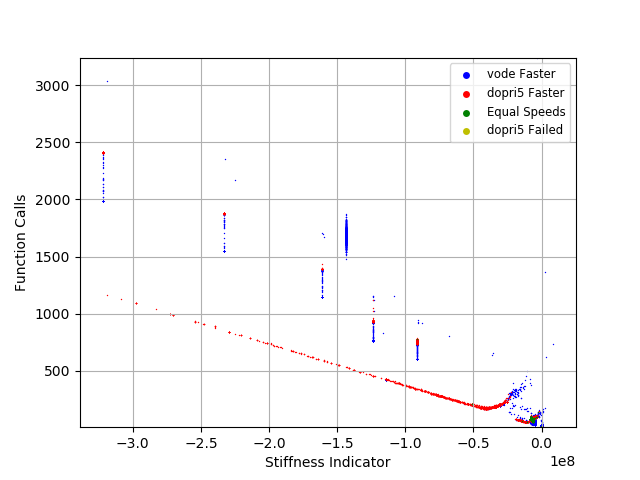
\includegraphics[width=\linewidth]{H2_CO/PaSR_Fn_Work_Indicator_Groupings_1e-06.png}
        \caption{Stiffness indicator versus the least function calls used to integrate one time-step at each particle of the PaSR model.}
        \label{fig:SI2H2COPaSR}
    \end{subfigure}
    \begin{subfigure}{0.43\textwidth}
        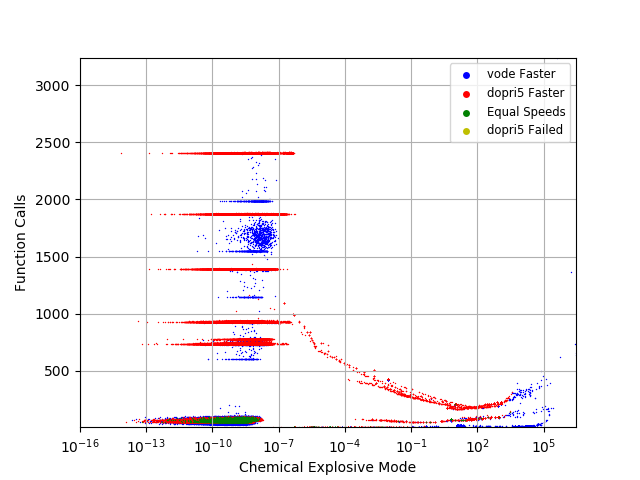
\includegraphics[width=\linewidth]{H2_CO/PaSR_Fn_Work_CEMA_Groupings_1e-06.png}
        \caption{Chemical explosive mode versus the least function calls used to integrate one time-step at each particle of the PaSR model.}
        \label{fig:CEMH2COPaSR}
    \end{subfigure}
    \caption{Stiffness metrics versus RHS function calls used to advance one time-step of the \ce{H2}\slash \ce{CO} model using either \texttt{vode} or \texttt{dopri5}.  Calculated with a constant step size of \SI{e-6}{\second} for every initial condition represented in the PaSR model.}
    \label{fig:H2COPaSRStiffness}
\end{figure}

As seen in Figure~\ref{fig:SRH2COPaSR}, the stiffness ratio was not highly correlated with the number of function calls required for either \texttt{vode} or \texttt{dopri5}, nor did it provide a particularly efficient indicator of the relative performance of either method.
\texttt{dopri5} outperformed \texttt{vode} at values of the stiffness ratio greater than $10^{19}$, however neither method had a clear advantage when values of the stiffness ratio were less than this.

The stiffness index had similar performance to the stiffness ratio, as seen in Figure~\ref{fig:SI1H2COPaSR}.
When the values of the stiffness index were less than $10^8$, \texttt{vode} typically outperformed \texttt{dopri5}.
At larger values of the stiffness index, neither method had a clear advantage.

The stiffness indicator had a better correlation with the number of function call used by either \texttt{vode} or \texttt{dopri5} than the other stiffness metrics, with a larger negative stiffness indicator correlating to a greater number of function calls as seen in Figure~\ref{fig:SI2H2COPaSR}.
Clear trends can be seen in plots of function calls versus the stiffness indicator values, which will be investigated in further research.
The stiffness indicator was less useful than the stiffness ratio or stiffness index at determining the relative speed of either method, as there is no clear correlation between the value of the stiffness indicator and the superiority of either method.

Similar to the stiffness ratio and the stiffness index, the chemical explosive mode was not highly correlated with the number of RHS function calls used.  \texttt{vode} outperformed \texttt{dopri5} when values of the chemical explosive mode were greater than $10^4$.

The PaSR data for GRI Mech 3.0 consisted of 450900 particles.  If I can ever get some data that tells me anything useful about these particles, I will be a happy man.

\begin{figure}[htbp]
   \centering
   \begin{subfigure}{0.43\textwidth}
       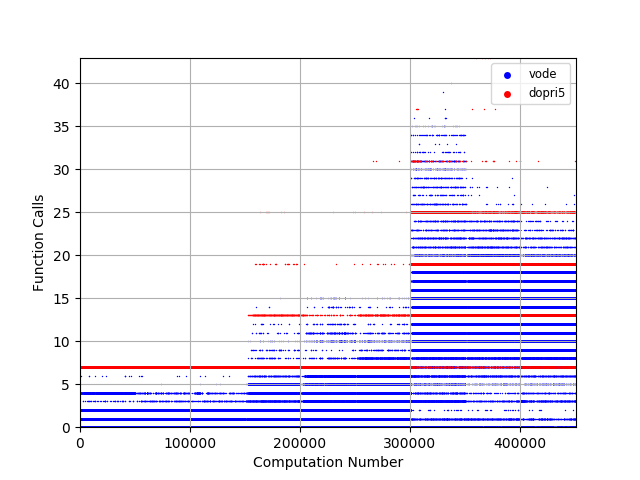
\includegraphics[width=\linewidth]{GRI_Mech_3/PaSR_Fn_Work_1e-09.png}
       \caption{Number of function calls used to integrate one time-step for both \texttt{dopri5} and \texttt{vode} at each particle of the PaSR model.}
       \label{fig:FWGRIPaSR}
   \end{subfigure}
   \hfill
   \begin{subfigure}{0.43\textwidth}
       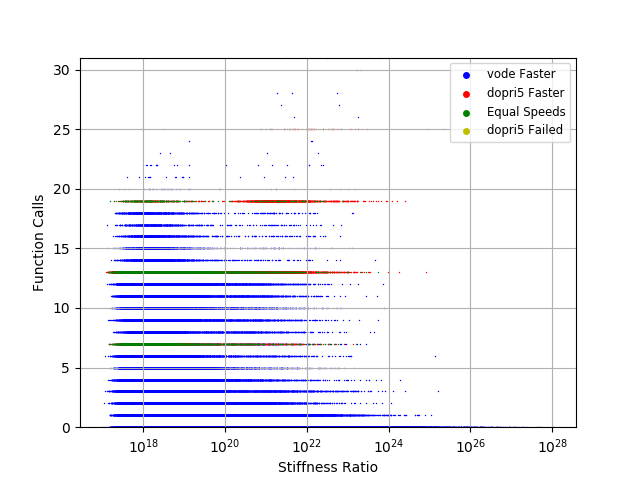
\includegraphics[width=\linewidth]{GRI_Mech_3/PaSR_Fn_Work_Ratio_Groupings_1e-09.png}
       \caption{Stiffness ratio versus the least function calls used to integrate one time-step at each particle of the PaSR model.}
       \label{fig:SRGRIPaSR}
   \end{subfigure}
   \begin{subfigure}{0.43\textwidth}
       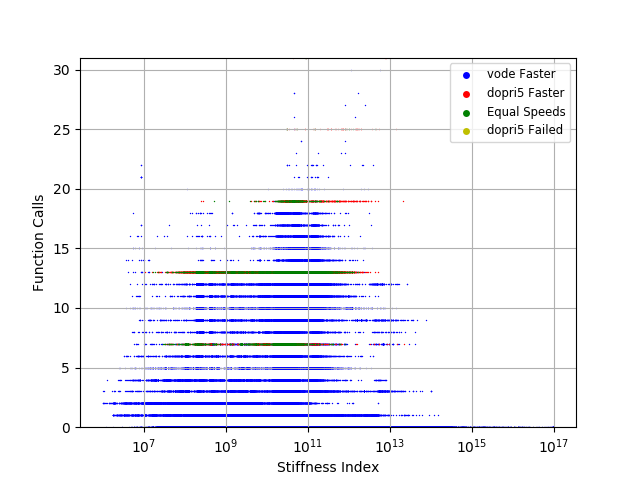
\includegraphics[width=\linewidth]{GRI_Mech_3/PaSR_Fn_Work_Index_Groupings_1e-09.png}
       \caption{Stiffness index versus the least function calls used to integrate one time-step at each particle of the PaSR model.}
       \label{fig:SI1GRIPaSR}
   \end{subfigure}
   \hfill
   \begin{subfigure}{0.43\textwidth}
       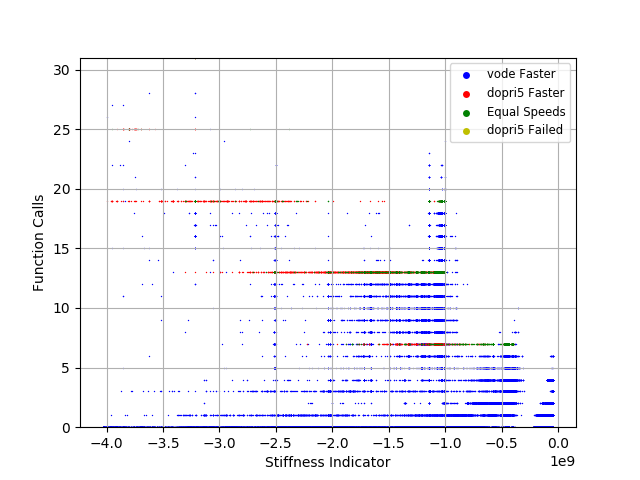
\includegraphics[width=\linewidth]{GRI_Mech_3/PaSR_Fn_Work_Indicator_Groupings_1e-09.png}
       \caption{Stiffness indicator versus the least function calls used to integrate one time-step at each particle of the PaSR model.}
       \label{fig:SI2GRIPaSR}
   \end{subfigure}
   \begin{subfigure}{0.43\textwidth}
       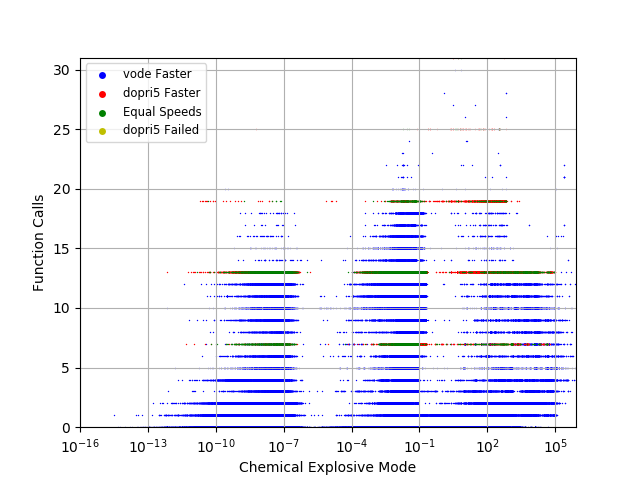
\includegraphics[width=\linewidth]{GRI_Mech_3/PaSR_Fn_Work_CEMA_Groupings_1e-09.png}
       \caption{Chemical explosive mode versus the least function calls used to integrate one time-step at each particle of the PaSR model.}
       \label{fig:CEMGRIPaSR}
   \end{subfigure}
   \caption{Stiffness metrics versus RHS function calls used to advance one time-step of the GRI Mech 3.0 model using either \texttt{vode} or \texttt{dopri5}.  Calculated with a constant step size of \SI{e-9}{\second} for every initial condition represented in the PaSR model.}
   \label{fig:GRIPaSRStiffness}
\end{figure}


\section{Conclusions}

Our analysis demonstrated that \texttt{dopri5} generally outperformed \texttt{vode} for the \ce{H2}\slash \ce{CO} model, especially when the pressure and initial temperature values were low.
%
% Our analysis demonstrated that the stiffness of the model prior to autoignition increases significantly during and after autoignition.
% This observation matches the expected behavior based on our intuition of the problem, but is based on a calculated metric.
% It also demonstrates the feasibility of using an explicit method prior to autoignition to save computational expense.
% Interestingly, we did not observe the maximum value of stiffness index during ignition; instead, this value occurred around \SI{0.02}{\second} after the reaching equilibrium (i.e., steady-state temperature and mass fractions).
% After reaching its maximum value, the stiffness remained relatively constant.
% The stiffness index evaluated provides a reasonable means of detecting the stiffness of combustion reactions.
% Incorporating calculation of this index in the code used to integrate the derivative vector will both accelerate calculation of the index and enable the index to be calculated on-the-fly.

\section{Acknowledgements}
This material is based upon work supported by the National Science Foundation under grant ACI-1535065.

\setlength{\emergencystretch}{3em}
\printbibliography


\end{document}
